\documentclass[11pt,a4paper,titlepage,twoside]{book}

%\usepackage[textwidth=450pt]{geometry}
\usepackage[left=1.38in,right=0in,top=1in,bottom=0.7in]{geometry}
\usepackage{graphicx}
\usepackage{lastpage}
\usepackage{fancyhdr}
\usepackage{pdfpages}
\usepackage{tikz}


%\usepackage{tabularx,makecell}


% %Options: Sonny, Lenny, Glenn, Conny, Rejne, Bjarne, Bjornstrup

\graphicspath{{figures/}}

\pagestyle{fancy}
\fancyhead{} 
\lhead{SPHERIC Beijing 2017}
\chead{}
\rhead{Workshop} 
\pagenumbering{gobble}

\begin{document}


\lhead{SPHERIC Beijing 2017}
\chead{}
\rhead{Workshop} 
\section*{Map of Peking University Campus}
\begin{tikzpicture}
\clip (-1\textwidth,-0.4812\textheight) rectangle(0,0.4812\textheight);
\node at (0,0){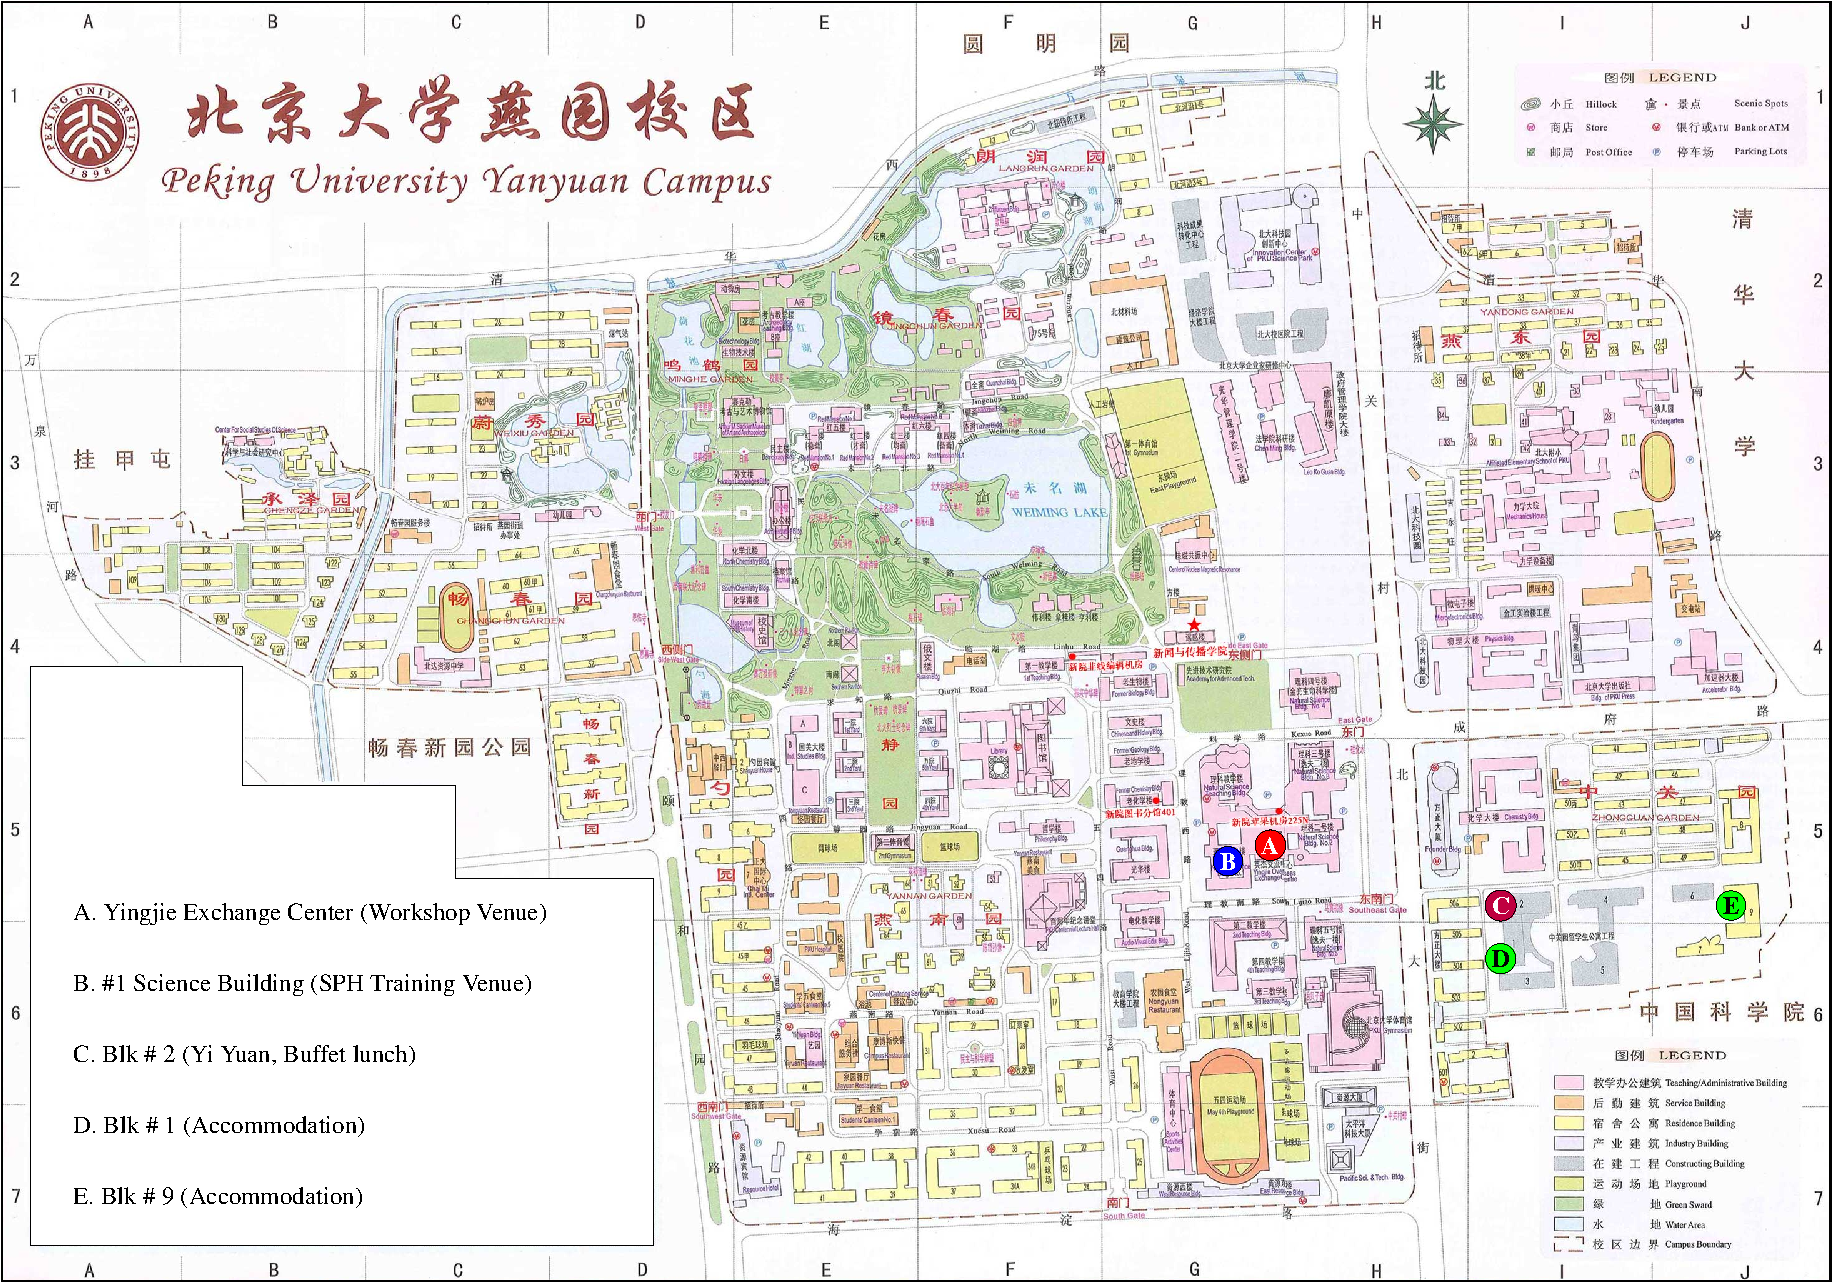
\includegraphics[width=2\textwidth]{PKU.pdf}};
\end{tikzpicture}


\newpage
\lhead{~Details}
\chead{}
\rhead{Map of Peking University Campus} 

\section*{\vphantom{Map of Peking University Campus}}
\begin{tikzpicture}
\clip (0,-0.4812\textheight) rectangle(1\textwidth,0.4812\textheight);
\node at (0,0){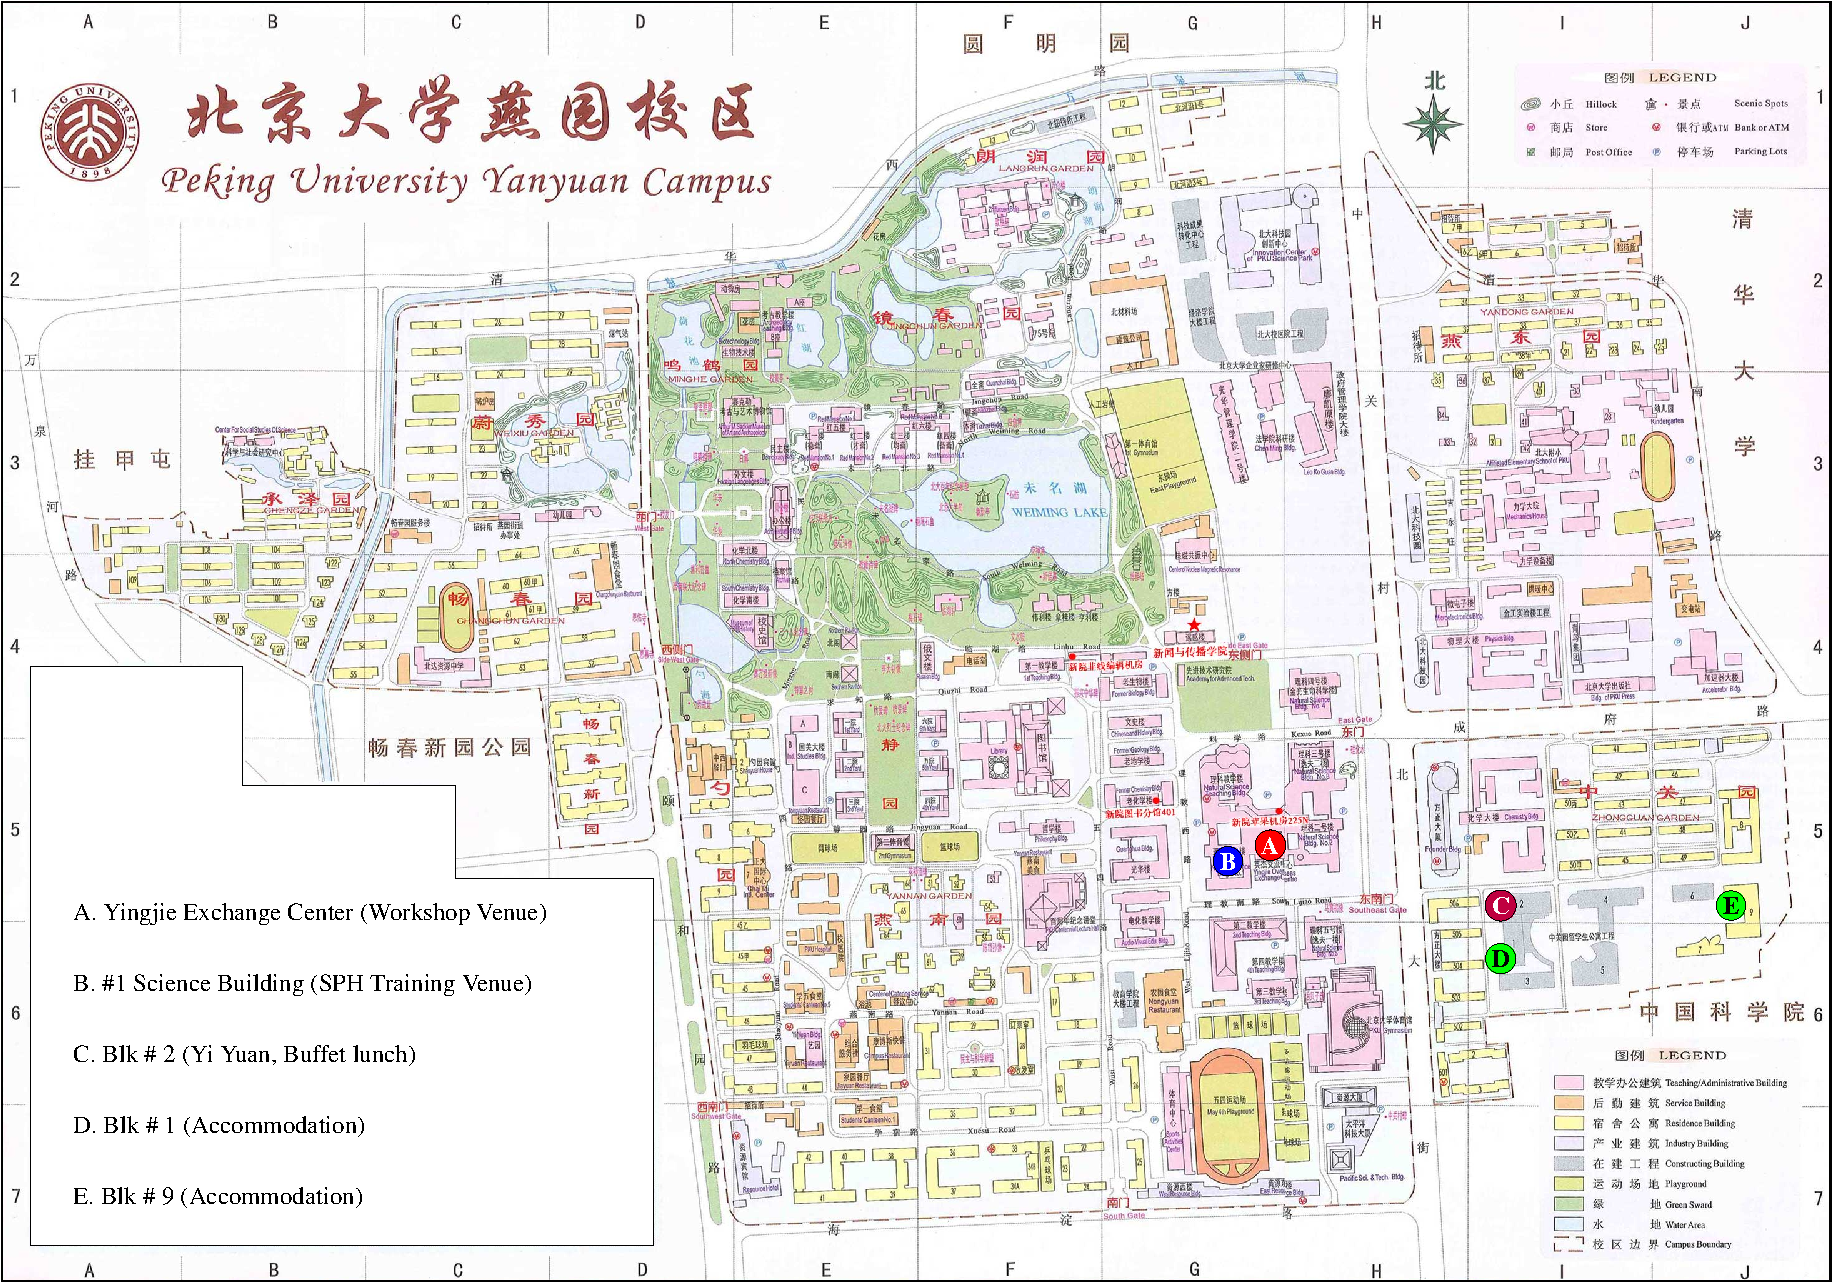
\includegraphics[width=2\textwidth]{PKU.pdf}};
\end{tikzpicture}








\end{document}